\documentclass[a4paper,11pt]{article}

\usepackage[frenchb]{babel}
\usepackage[utf8]{inputenc}
\usepackage{verbatim}
\usepackage{graphicx}

\begin{document}

\title{Compte Rendu du TD numéro 5 de l'équipe Eirb'reteau}
\date{TD du 17 octobre, pour le 21 octobre}
\maketitle

\begin{center}
  Coordinateur :  Pierre Gaulon\\
  Tandem 1 : Aurélien Nizet, Lionel Adotevi\\
  Tandem 2 : Reda Boudjeltia, Victor Dury\\
\end{center}

\section{Relation de type/sous-type}
Dans cette section, nous allons établir des relations de type/sous-type pour les deux nouveaux caractères de passagers que nous allons créer.

Nous avons besoin d'un héritage de classe pour éviter de dupliquer le code. En effet, les trois types de passagers (lunatique, stressé et standard) auront notamment les mêmes attributs, puisque seul leur comportement, à la montée ou à un arrêt, change. Pour factoriser le code, il est nécessaire de mettre ces attributs, entre autres, dans une classe mère à ces trois caractères. Cela ne peut pas être fait avec une interface, qui ne peut pas contenir d'attributs. Il n'est donc pas possible d'utiliser seulement un héritage d'interfaces dans cet objectif de factorisation de code.

L'objectif de garder Passager sans code est de définir un comportement minimal, une sorte de cahier des charges que devront respecter tous les passagers. Garder Passager sans code est en faveur de l'abstraction. Le Passager va donc rester indépendant de sa réalisation.

Dans l'exemple du cours, c'est un lien a-un qui est utilisé. La classe Verrou contient des instances des classes PorteCharniere et PorteCoulissante, et il applique ses méthodes sur ces instances. En fait, ces instances sont déclarées du type de leur classe mère, la classe Porte. Ainsi, les mécanismes de polymorphisme se chargent du reste.

En utilisant la solution de relation de type/sous-type, et non de lien a-un, l'objectif est toujours le même : l'abstraction, rendre les objets les plus indépendants les uns des autres en favorisant l'encapsulation.

\section{L'héritage de classe}
Nous rassemblons maintenant le code commun à toutes les classes, dans une classe nommée PassagerAbstrait, sous-type de Passager et Usager. Les classes PassagerStandard, PassagerStresse et PassagerLunatique en héritent.

\begin{figure}[!ht]
  \begin{center}
    \caption{Diagramme de classes}
    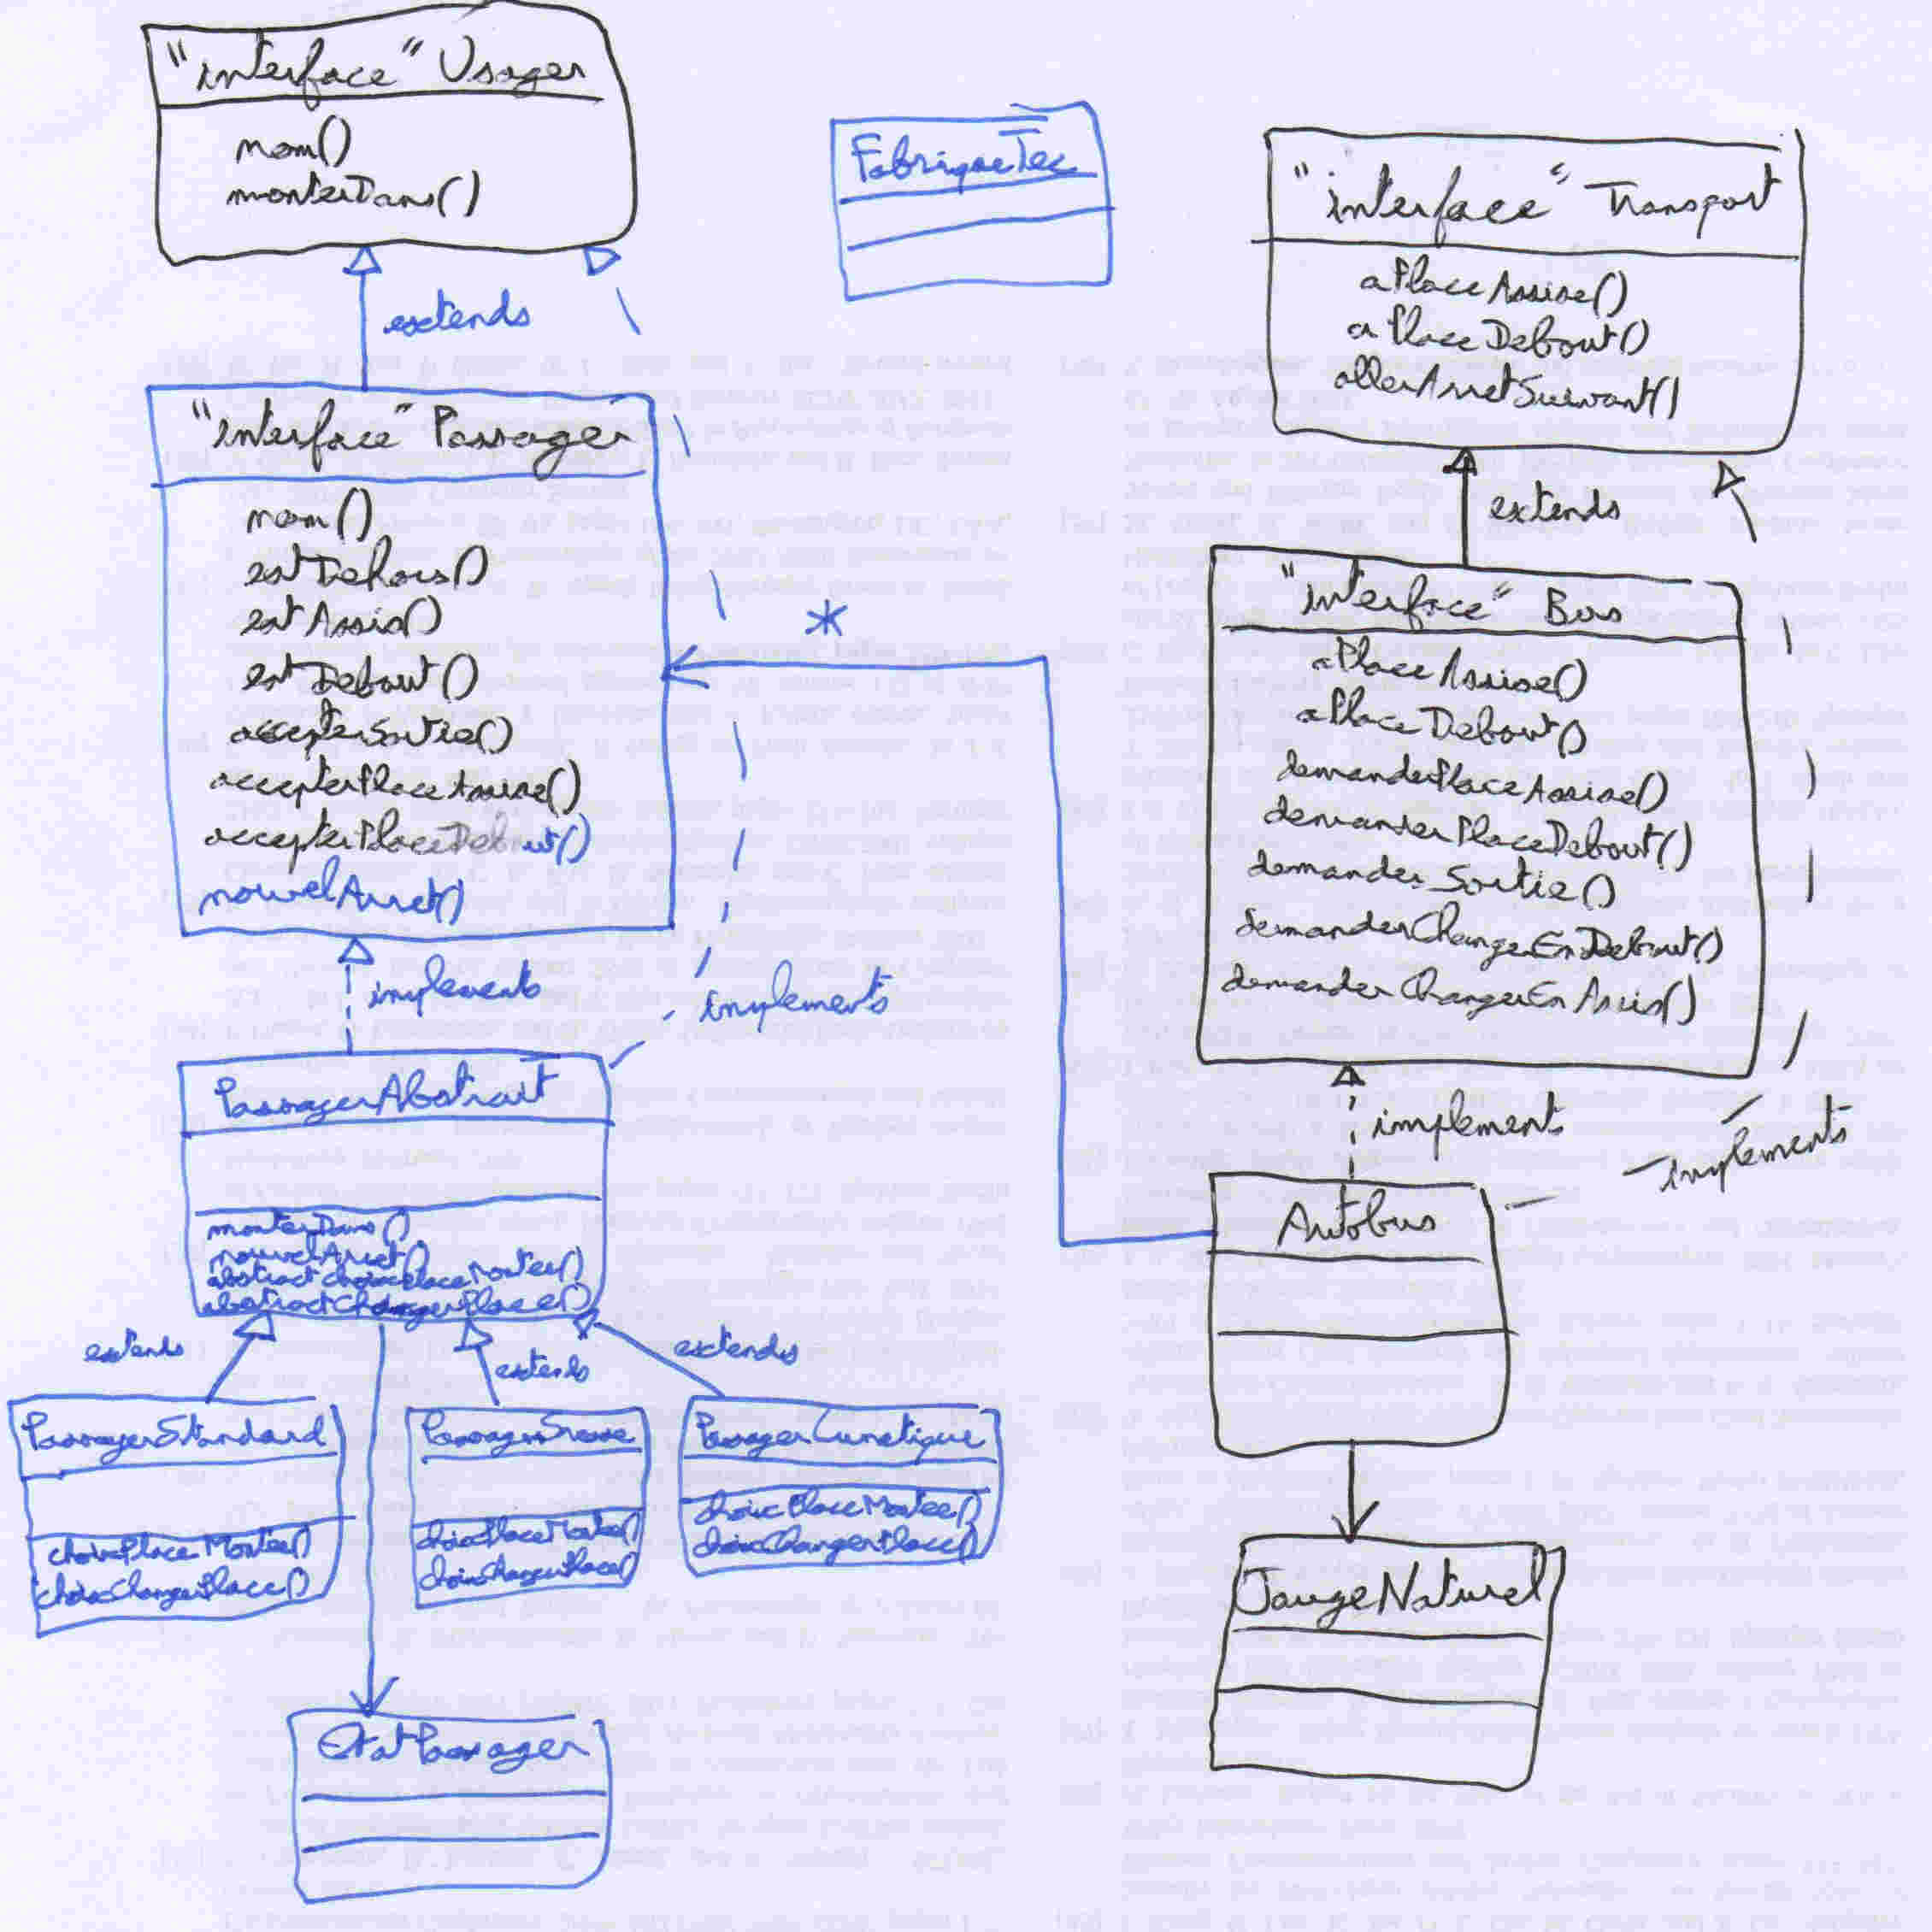
\includegraphics[scale=0.1]{diagramme.jpg}
  \end{center}
\end{figure}

\subsection{La classe PassagerAbstrait}
Cette classe PassagerAbstrait implémente l'interface Passager et l'interface Usager, où sont contenues les méthodes monterDans() et nouvelArret(). Or, ces méthodes ne figurent pas dans PassagerAbstrait, puisqu'elles sont supprimées de cette classe. Une méthode qui ne définit pas toutes les méthodes des interfaces qu'elle implémente, qui est incomplète, doit être abstraite. En effet, elle ne doit pas pouvoir être instanciée, puisqu'il reste des méthodes sans code.

Cette classe abstraite PassagerAbstrait possède un constructeur car ce constructeur peut être utilisé par les classes filles pour initialiser les attributs de la classe mère, peut-être même en utilisant des méthodes de la classe mère. Cela n'aurait pas été possible sans constructeur dans cette classe abstraite, même si elle n'est pas instanciable.

\subsection{La classe PassagerStandard}
La classe PassagerStandard est remaniée, de façon à hériter de la classe PassagerAbstrait, et à définir le comportement standard pour les méthodes monterDans() et nouvelArret().

Si on définit la portée de la variable destination en protected, cela signifie qu'elle est accessible dans le paquet tec. Ainsi, cette variable de la classe PassagerAbstrait peut être modifiée par d'autres classes du paquet tec. L'encapsulation n'est donc pas respectée.

Si le constructeur PassagerStandard() est vide, alors que cette classe hérite de PassagerAbstrait, le code vide va être remplacé par l'appel à super(), sans paramètres. La méthode super() se référant au constructeur de la classe PassagerAbstrait, qui compte deux paramètres, il va y avoir une erreur, indiquant qu'il manque des paramètres dans ce constructeur.

Il est obligatoire de déclencher un constructeur de la classe de base avant celui de la classe dérivée, car les attributs de la classe de base sont initialisés avant ceux de la classe dérivée, et le code du constructeur de la classe dérivée peut utiliser des méthodes de la classe de base.

\subsection{Les deux nouveaux caractères}
Le code en commun entre les classes PassagerStandard, PassagerLunatique et PassagerStresse est contenu dans les deux méthodes nouvelArret() et monterDans() de PassagerAbstrait :
\begin{itemize}
\item Dans nouvelArret(), on trouve le code
\begin{verbatim}
if( destination == numeroArret )
bus.demanderSortie(this);
\end{verbatim}
\item Dans monterDans(), on trouve le cast
\begin{verbatim}
Bus b = (Bus) t;
\end{verbatim}
\end{itemize}

\section{Définir ce qu'il faut paramétrer}
Nous allons mettre dans la classe PassagerAbstrait le code dupliqué, afin de le factoriser. Pour ce faire, il faut transferer les méthodes nouvelArret() et monterDans() dans la classe abstraite, et y déclarer deux nouvelles méthodes abstraites choixPlaceMontee() et choixChangerPlace(), que chacune des classes dérivée définira selon le comportement souhaité.

C'est le mécanisme de polymorphisme qui va se charger d'aiguiller correctement les méthodes choixChangerPlace() et choixPlaceMontee() vers la bonne classe. Cette liaison est dynamique, elle se fait à l'exécution du programme en fonction de l'instance manipulée, pour obtenir l'adresse de la méthode à l'exécution.

\subsection{La classe PassagerAbstrait}
Les deux nouvelles méthodes choixPlaceMontee() et choixChangerPlace() sont des méthodes abstraites.
Si on met un corps vide pour ces deux méthodes, on sera alors obligés de les réécrire dans les classes dérivées (@Override), alors que si on laisse seulement la signature de ces méthodes (méthodes abstraites), on laisse alors le soin à chaque classe dérivée de définir ces méthodes comme elle l'entend, sans la réécrire.
Ces deux méthodes ont une portée publique par défaut.

Pour s'assurer que les méthodes monterDans() et nouvelArret() ne soient redéfinies, il faut ajouter le mot-clé final à ces deux méthodes. Elles ne pourront ainsi pas être réécrites.

\subsection{Les classes caractères}
Nous écrivons maintenant le code des classes PassagerStresse, PassagerLunatique, et PassagerStandard, ainsi que leurs tests.

Ces classes de caractères doivent être déclarées final, pour qu'aucune autre classe n'en hérite. Ces classes de caractères sont les classes de plus bas niveau, c'est-à-dire qu'il n'est pas envisageable qu'il y ait de sous-caractères ou aucune autre classe qui en dérive. Cela empêche ainsi tout utilisation inappropriée de ces classes.

\section{Factoriser les tests}
Le classe TestPassagerAbstrait est définie abstraite, et possède une méthode abstraite servant de constructeur, qui est redéfinie dans chaque classe dérivée TestPAssagerStandard, TestPassagerLunatique et TestPassagerStresse. Le type de retour utilisé est PassagerAbstrait, puisque d'une part nous voulons seulement tester les PassagersAbstraits, et non les Passagers ou les Usagers, et d'autre part, parce que ces deux derniers sont des interfaces, et non des classes à instancier.

\section{Commentaires}
\subsection{Commentaire de Pierre}
Je pense que les deux notions importantes à tirer de ce TD sont l'encapsulation et la factorisation de code. En effet, il y a une marge entre produire un code qui fonctionne, et produire un code bien pensé, propre et concis. C'est cette approche qui nous a été suggérée ici, notamment par le fait de créer beaucoup de classe, mais que chacune ait un rôle bien particulier et propre, l'encapsulation, et par le fait de créer des classes abstraites pour factoriser le code. Le but étant d'avoir un code facilement maintenable pour gagner du temps par la suite. Ici, on s'est donc abstraits des problèmes techniques du langage en lui-même, pour s'intresser plutôt aux fondements de la programmation orientée objet.

\subsection{Commentaire d'Aurélien}
Ce TD consistait à créer la classe abstraite PassagerAbstrait ainsi que les classes PassagerLunatique et PassagerStresse. Bien que le code à écrire n'était pas conséquent, il a fallu bien faire attention lors de la factorisation du code et ainsi remanier correctement le code des fichiers sources ainsi que des fichiers tests. Je me suis également rendu compte dans ce TD que ce n'est pas simple de fournir du code bien factorisé, avec des tests unitaires également factorisés. Mais le fait est qu'une fois le code correctement écrit, il est alors beaucoup plus facile de modifier par exemple une fonction bien précise sans avoir à retoucher tout le code !

\subsection{Commentaire de Reda}
Dans ce TP, j'ai appris à faire évoluer des classes afin de les rendre plus réalistes (les types de passagers). Grâce au système d'héritage sur les classes abstraites cela se fait plutôt simplement. De plus, j'ai pu découvrir l'utilisation et l'intérêt des exceptions.

\subsection{Commentaire de Victor}
J'ai trouvé ce TD agréable car nous avons pu voir l'abstraction de plusieurs classes en une classe pour éviter le code commun. Nous nous doutions que nous pouvions faire une telle chose, mais nous avons pu constater que ça fonctionnait bien.

\subsection{Commentaire de Lionel}
Ce TD était pour moi un approfondissement des notions d'héritage, d'abstraction mais aussi un plus sur la factorisation de code et l'importance des tests
unitaires. Cela montre les différentes étapes à respecter lors de l'écriture
d'un code.

\end{document}
